\chapter{Задание № 1}
\section{Текст программы по индивидуальному варианту}
Текст программы по индивидуальному варианту приведён на листинге \ref{programText}
\begin{lstlisting}[label=programText,caption=Текст программы по индивидуальному варианту]
	.section .text
	.globl _start;
	len = 8
	enroll = 1 
	elem_sz = 4 
	
	_start:
	la x1, _x                       // into x1 beginning of mas
	addi x20, x1, elem_sz*(len-1)   // x20 = x1 + (len - 1) * size
lp:
	lw x2, 0(x1)                    // x2 = x1[0]
	addi x1, x1, elem_sz*enroll #!  // x1 += elem_sz;
	add x31, x31, x2                // x31 += x2;
	bne x1, x20, lp                 // if (x1 != x20) goto lp;
	addi x31, x31, 1                // x31 += 1
	lp2: j lp2
	
	.section .data
	_x:     .4byte 0x1
	.4byte 0x2
	.4byte 0x3
	.4byte 0x4
	.4byte 0x5
	.4byte 0x6
	.4byte 0x7
	.4byte 0x8
\end{lstlisting}

\section{Дизассемблерный листинг кода программы}
В результате выполнения компиляции был создан файл с расширением .hex, хранящий содержимое памяти команд и данных. В окне терминала отобразился дизассемблерный листинг, который приведён в листинге \ref{img:var4disassembler}.

\begin{figure}[H]
	\begin{center}
		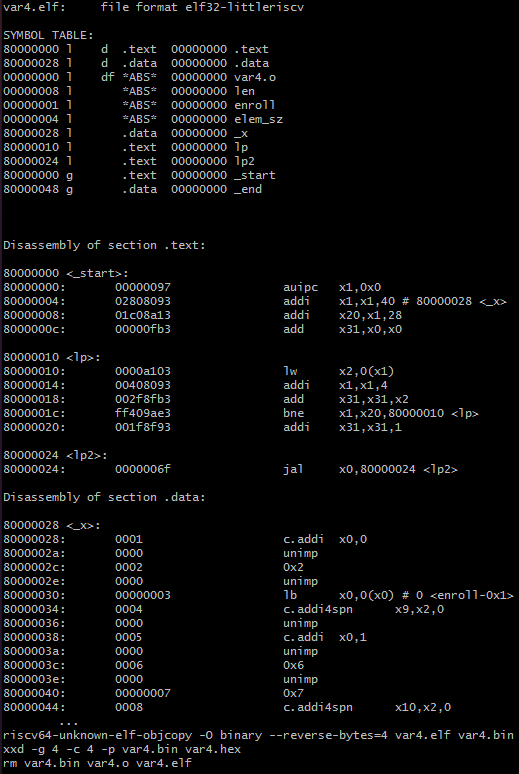
\includegraphics[scale=0.65]{img/var4disassembler.png}
	\end{center}
	\captionsetup{justification=centering}
	\caption{Скриншот дизассемблированной программы по варианту}
	\label{img:var4disassembler}
\end{figure}

\section{Псевдокод, поясняющий работу программы}
В рисунке \ref{img:var4pseudocode} и листинге \ref{pscode} приведён псевдокод, поясняющий работу программы.
\begin{figure}[H]
	\begin{center}
		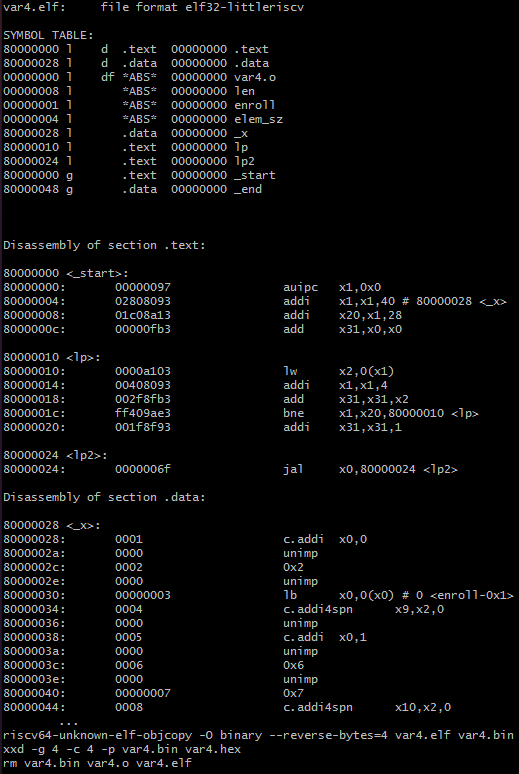
\includegraphics[scale=0.65]{img/var4disassembler.png}
	\end{center}
	\captionsetup{justification=centering}
	\caption{Скриншот псеводкода на языке С, поясняющего работу программы}
	\label{img:var4pseudocode}
\end{figure}

\begin{lstlisting}[extendedchars=\true, keepspaces=true, escapechar=\%,
	texcl=\true, label=pscode,caption=Псевдокод, поясняющий работу программы]
	1. Инициализация массива _x, состоящего из 8 элементов, значениями от 1 до 8 включительно. Каждое значение по 4 байта.
	2. Инициализация параметров алгоритма:
	len = 8
	enroll = 1 
	elem_sz = 4
	3. Установка указателя x1 на начало массива:
	x1 = _x
	4. Вычисление указателя на последний элемент массива:
	x20 = x1 + (len - 1) * size
	5. Цикл: пока x1 не равно x20
	5.1. x2 = x1[0]
	5.2. x1 = x1 + elem_sz * enroll
	5.3. x31 = x31 + x2
	6. x31 = x31 + 1
\end{lstlisting}

Очевидно, что в регистре x31 после выполнения программы должно содержаться значение:
\begin{displaymath}
	x31 = \sum\limits_{i=1}^7{i} + 1 = 29.
\end{displaymath}
\newpage

\chapter{Задание №2}
\section{Выполнение}
В результате симуляции, был получен снимок экрана, содержащий временную диаграмму выполнения стадий выборки и диспетчеризации команды с адресом 80000018 (1 итерация). Снимок экрана приведён на рисунке \ref{var4fetch}.

\begin{figure}[h!p]
	\centering
	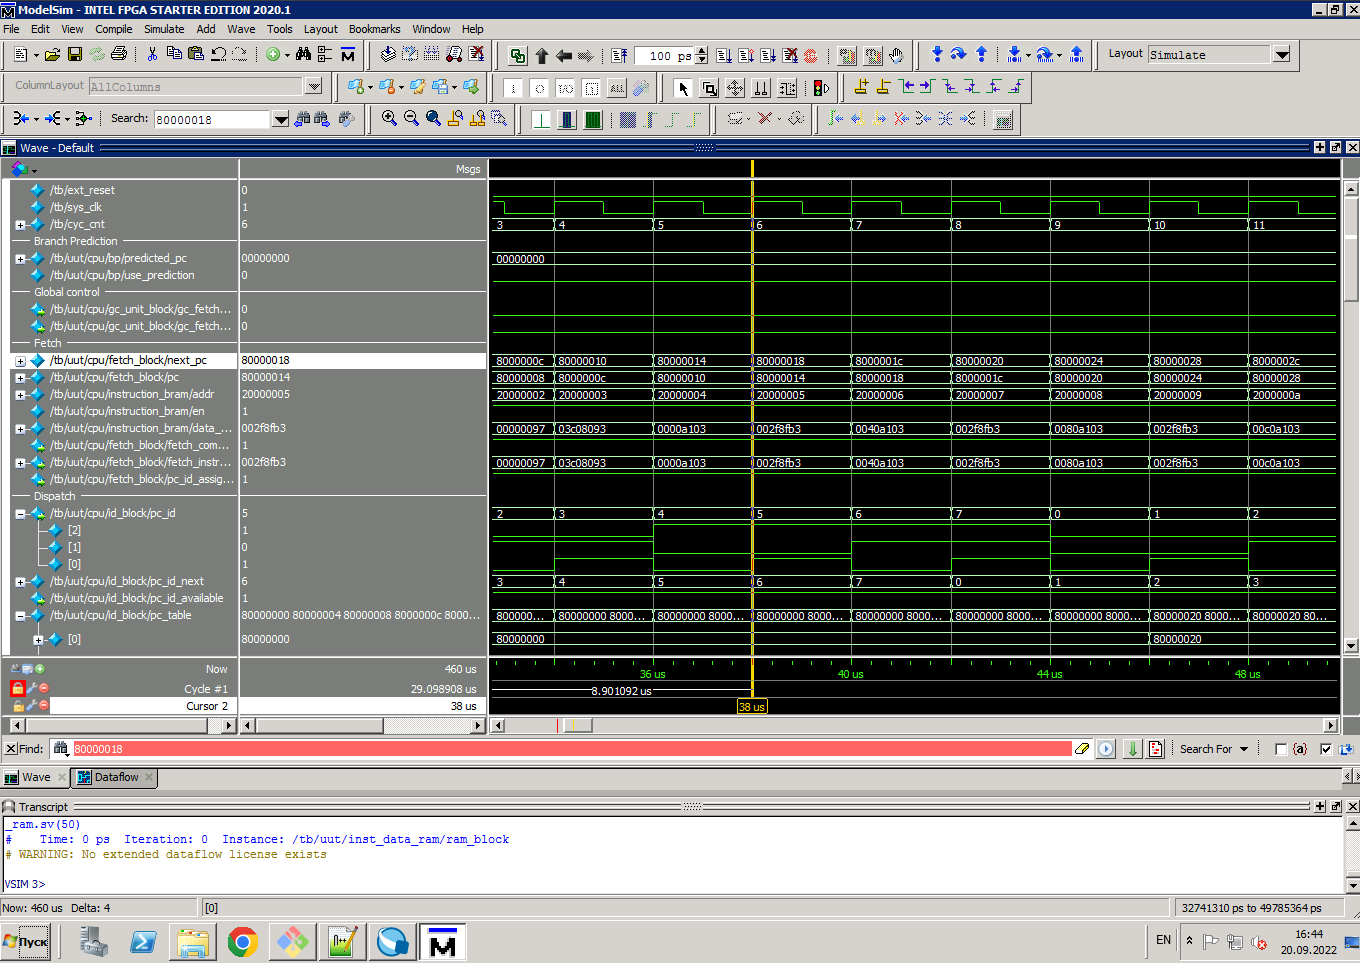
\includegraphics[width = \linewidth]{img/var4fetch.png}
	\caption{Временная диаграмма выполнения стадий выборки и диспетчеризации команды с адресом 80000018 (1 итерация)}
	\label{var4fetch}
\end{figure}
Рассмотрим происходящее на рисунке \ref{var4fetch}. Будем называть первым тактом самый левый такт на рисунке.
\begin{itemize}
	\item На 1 такте \verb|pc| = 80000018. Этот адрес выставляется на ША памяти команд (причём адрес получается с помощью деления на 4, так как память в RISC-V адресуется в байтах, а память команд адресуется блоками по 4 байта). Таким образом, \verb|instruction_bram/addr| = 20000006. Идентификатор команды (\verb|pc_id|) присваивается в момент начала выборки, то есть одновременно с выставлением адреса команды на ША памяти команд. Кроме того, по фронту \verb|clk|, завершающему такт адрес команды(то есть, значение регистра \verb|pc| на момент выборки) записывается в таблицу \verb|pc_table| по присвоенному идентификатору.  
	\item На 2 такте память команд выдает данные (то есть, код команды), прочитанные по адресу, который был выставлен на ША в предыдущем такте (сигнал \verb|data_out|). Блок выборки выдает эти данные на линию \verb|fetch_instruction|. Устанавливается сигнал \verb|fetch_complete|, подтверждающий выборку и наличие кода команды на линии \verb|fetch_ins|-\verb|truction|. В \verb|pc| записывается адрес следующей команды.
	\item На 3 такте код команды записывается в таблицу \verb|instruction_table| по идентификатору, который был присвоен ранее.
\end{itemize}


\chapter{Задание №3}
\section{Выполнение}
После того, как на выходе блока управления метаинформацией сформирован пакет данных, описывающих очередную инструкцию (то есть, поле decode.valid принимает значение 1) начинается этап
декодирования этой инструкции и планирования ее на выполнение. Данный этап выполняется блоком декодирования и планирования на выполнение.

В результате симуляции, был получен снимок экрана, содержащий временную диаграмму выполнения стадии декодирования и планирования на выполнение команды с адресом 80000024 (1 итерация). Снимок экрана приведён на рисунке \ref{var4task3}.

\begin{figure}[h!p]
	\centering
	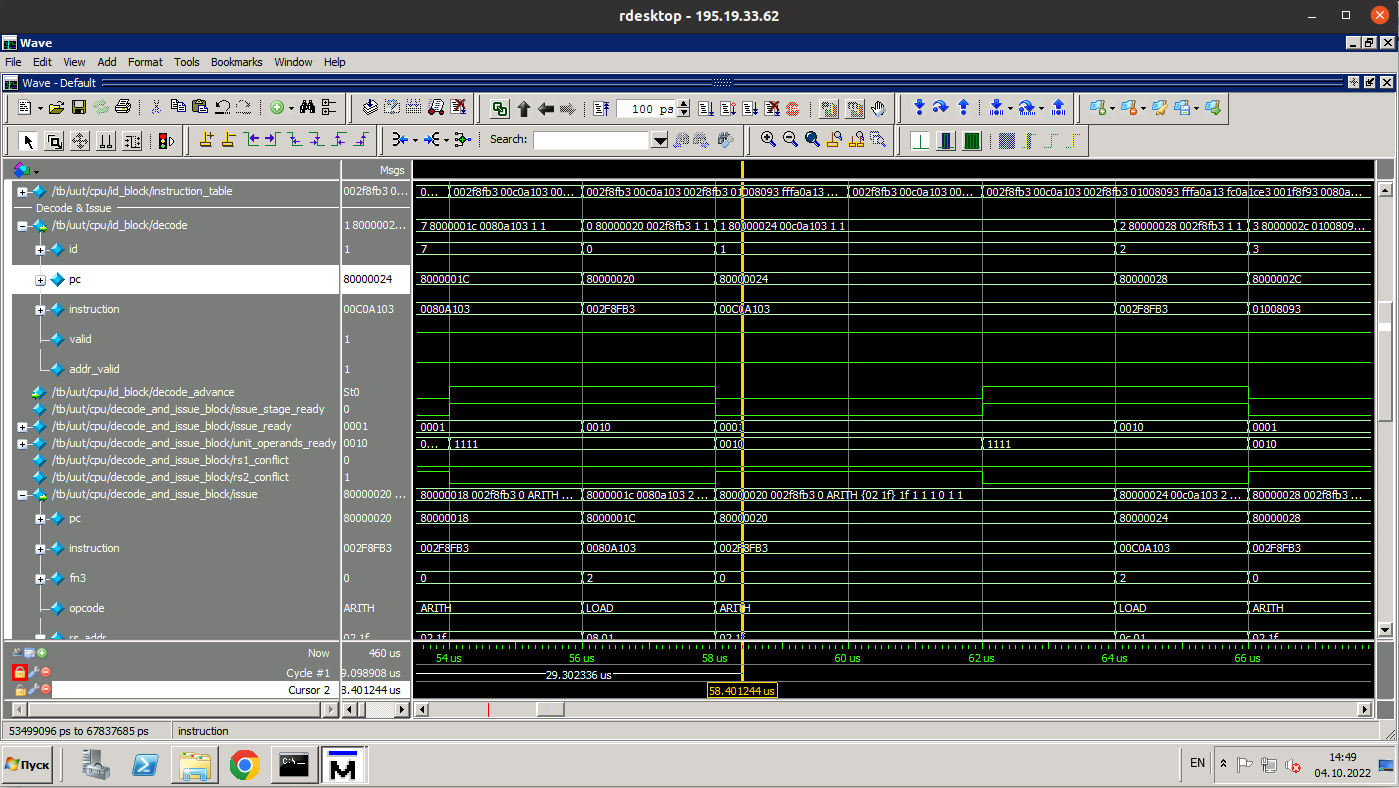
\includegraphics[width = \linewidth]{img/var4task3.png}
	\caption{Временная диаграмма выполнения стадии декодирования и планирования на выполнение команды с адресом 80000024 (1 итерация)}
	\label{var4task3}
\end{figure}

Рассмотрим происходящее на рисунке \ref{var4task3}. Будем называть первым тактом самый левый такт на рисунке.
\begin{itemize}
	\item В такте, предшествующем первому, происходит диспетчеризация команды с id=1. В такте 1 она поступает на вход блока декодирования (это видно по тому признаку, что сигнал decode.valid установлен).
	\item В такте 1 происходит декодирование команды. Команда не может быть запланирована на выполнение, так как занято устройство LSU (блок управления памятью, выполняющий команду), поэтому проходит 2 такта ожидания. При освобождении блока управления памятью устанавливается сигнал \verb|decode_advance| для передачи блоку управления метаинформацией указания выдать очередную команду для декодирования в следующем такте.
	\item В начале такта 4 выдаются сигналы для исполнительных блоков. На основании сигнала \verb|issue| формируются сигналы \verb|rs1_conflict|, \verb|rs2_conflict| равные 0, так как конфликта по регистрам нет. Отсутствие конфликта дает возможность точно выполнить данную команду в этом такте, соответственно сигнал \verb|decode_advance| должен быть установлен в 1.
\end{itemize}

\chapter{Задание №4}
\section{Выполнение}
После того, как команда запланирована для выполнения и нет конфликта по регистрам, начинается этап выполнения команды каким-либо исполнительным блоком. Однако, в начале этапа выполнения происходит чтение исходных регистров команды, информация о которых содержится в сигнале issue. Чтение регистрового файла выполняется комбинационно, то есть, данные на выходе регистрового файла выдаются в том же такте, что и сигнал issue.

В результате симуляции, был получен снимок экрана, содержащий временную диаграмму выполнения стадии выполнения команды с адресом 8000000c (1 итерация). Снимок экрана приведён на рисунке \ref{var4task4}.

\begin{figure}[h!p]
	\centering
	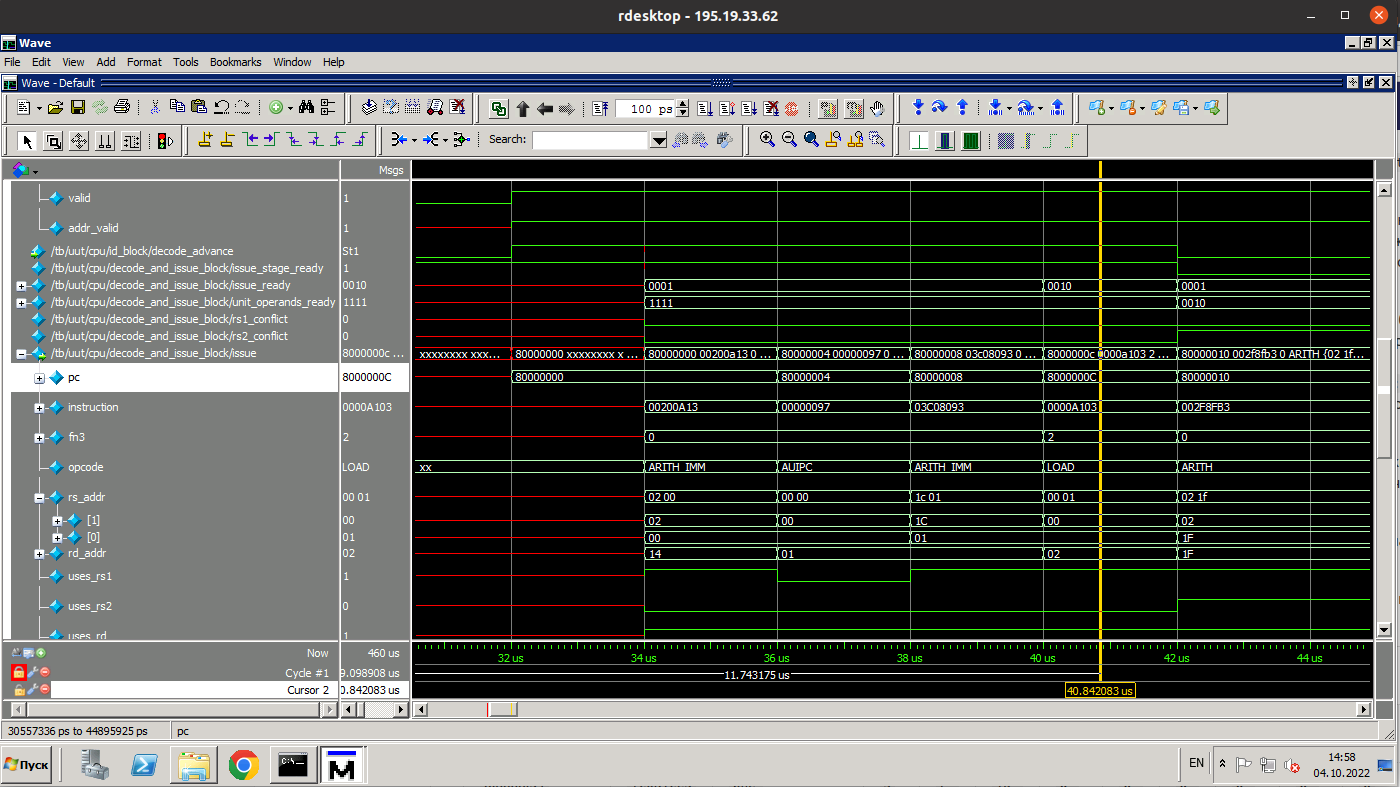
\includegraphics[width = \linewidth]{img/var4task4.png}
	\caption{Временная диаграмма выполнения стадии декодирования и планирования на выполнение команды с адресом 8000000с (1 итерация)}
	\label{var4task4}
\end{figure}

Рассмотрим происходящее на рисунке \ref{var4task4}. Видно, что команда будет обработана блоком обращения к памяти.
\begin{itemize}
	\item В момент планирования на выполнение новой команды (то есть, в момент выставления сигнала \verb|unit_issue[1].new_request|) происходит формирование на основе сигнала \verb|ls_inputs| атрибутов транзакции доступа к памяти (адрес, тип, размер и пр.) и их запись в очередь транзакций.
	\item В следующем такте характеристики транзакции становятся доступны на выходе очереди транзакций (сигнал \verb|transaction_out|), что подтверждается сигналом \verb|transaction_|-\verb|ready|. Выполняется дешифрирование адреса и определение вида памяти к которой происходит доступ. Готовность памяти данных (в нашем случае, готовность памяти имеется всегда, так как время доступа к памяти всегда составляется 1 такт) дает возможность сформировать запрос к памяти, то есть выставить на ША адрес, соответствующий характеристикам транзакции. Адрес формируется комбинационно. Так как блок рассчитан на работу с памятью с неизвестной заранее задержкой, то характеристики запроса к памяти записываются в очередь запросов к памяти.
	\item В следующем такте память данных выставляет на ШД прочитанные данные (сигнал \verb|data_out_b|) и сигнал готовности данных \verb|data_valid|. Блок фиксирует выполнение команды выставлением сигнала \\
	\verb|unit_wb[1].done| (формируется комбинационно по сигналу \verb|data_valid|), \verb|unit_wb[1].id| (берется из выхода очереди запросов к памяти) и \verb|unit_wb[1].rd| (берется с ШД памяти данных). В этом же такте происходит запись в целевой регистр. 
\end{itemize}

Таким образом видно, что выполнение команды доступа к памяти занимает минимум 3 такта.


\chapter{Задание №5}
В заданиях 2-4 симуляция проводилась на программе из примера. В задании №5 симуляция проводится на программе из индивидуального варианта, которая описана в 1 задании. 

\section{Сравнение полученного теоретически значения регистра x31 и полученного в результате симуляции}
Для проверки сравним значение регистра x31, вычисленного теоретически, с полученным в результате симуляции. Теоретически было получено значение 29. Результат симуляции представлен на рисунке \ref{var4task5_01}. Видим, что значения совпадают, так как ${1D}_{16} = {29}_{10}$

\begin{figure}[h!p]
	\centering
	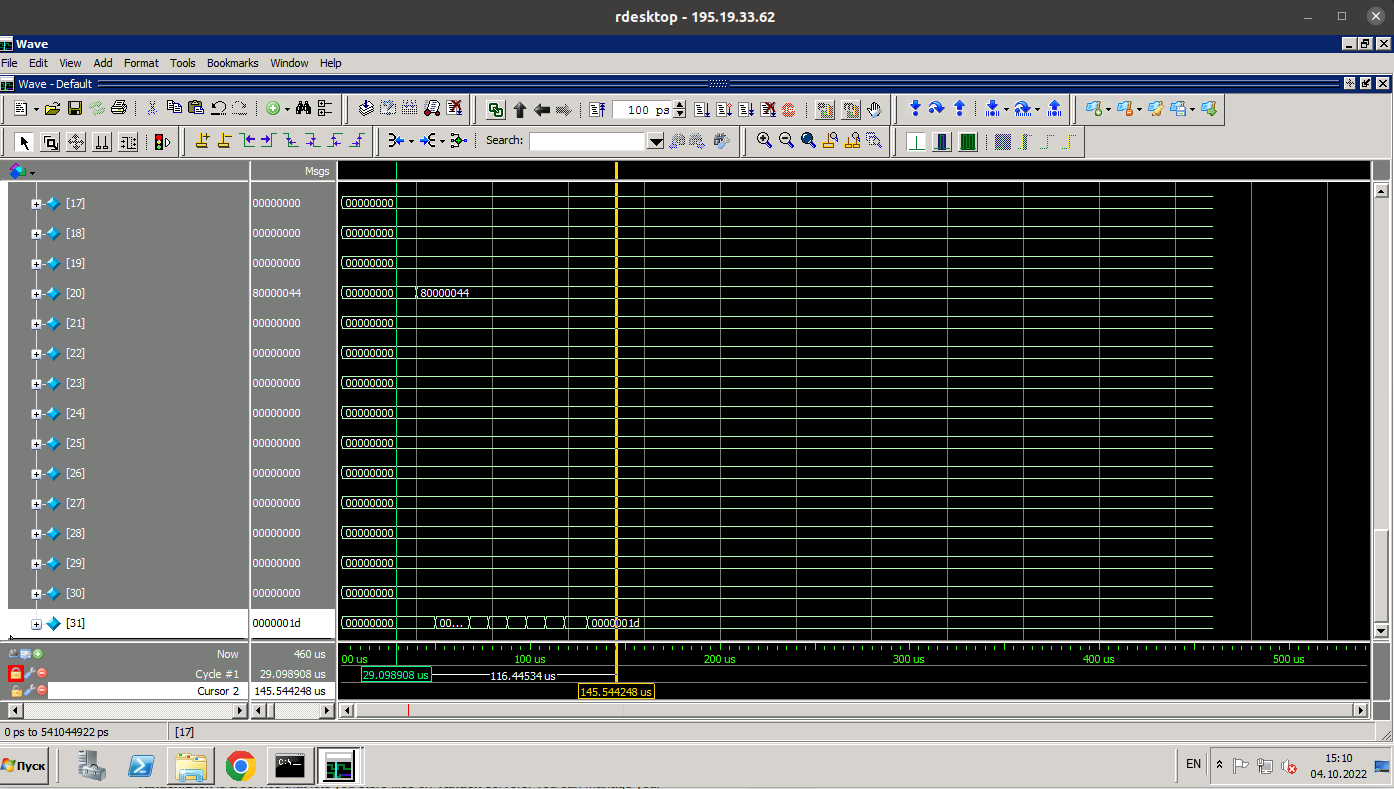
\includegraphics[width = \linewidth]{img/var4task5_01.png}
	\caption{Значение регистра x31, полученное в результате симуляции}
	\label{var4task5_01}
\end{figure}

\section{Временные диаграммы сигналов, соответствующих всем стадиям выполнения команды 80000010}
В тексте программы \ref{programText} символом \verb|#!| обозначена команда \verb|addi| \verb|x1|, \verb|x1|, \verb|elem_sz| * \verb|enroll|. Из дизассемблерного листинга кода программы \ref{img:var4disassembler} очевидно, что эта команда имеет адрес \verb|80000010|.

На рисунках \ref{var4task5fetch} и \ref{var4task5decode} приведены временные диаграммы сигналов, соответствующих всем стадиям выполнения команды с адресом 80000010.
\begin{figure}[h]
	\centering
	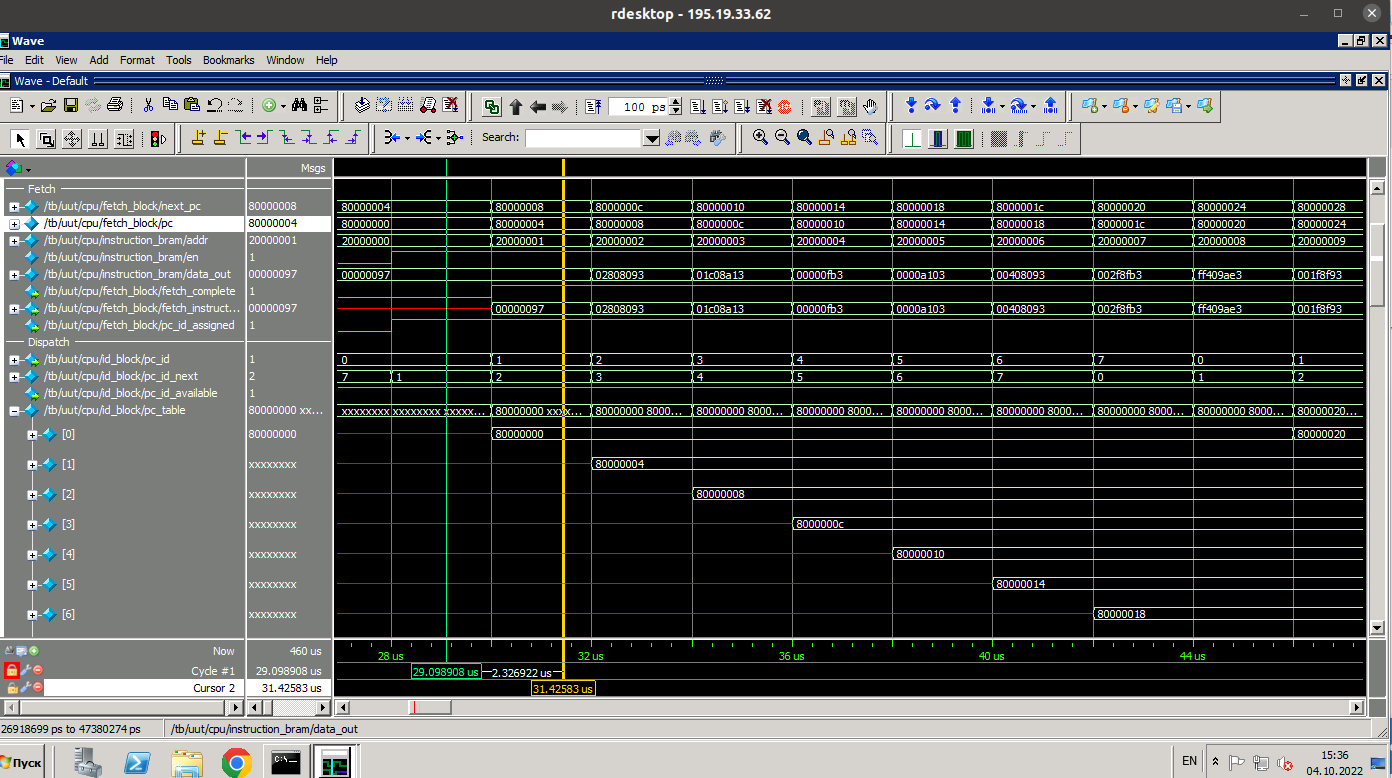
\includegraphics[width = \linewidth]{img/var4task5fetch.png}
	\caption{Временная диаграмма выполнения стадий выборки и диспетчеризации команды с адресом 80000010}
	\label{var4task5fetch}
\end{figure}

\begin{figure}[h]
	\centering
	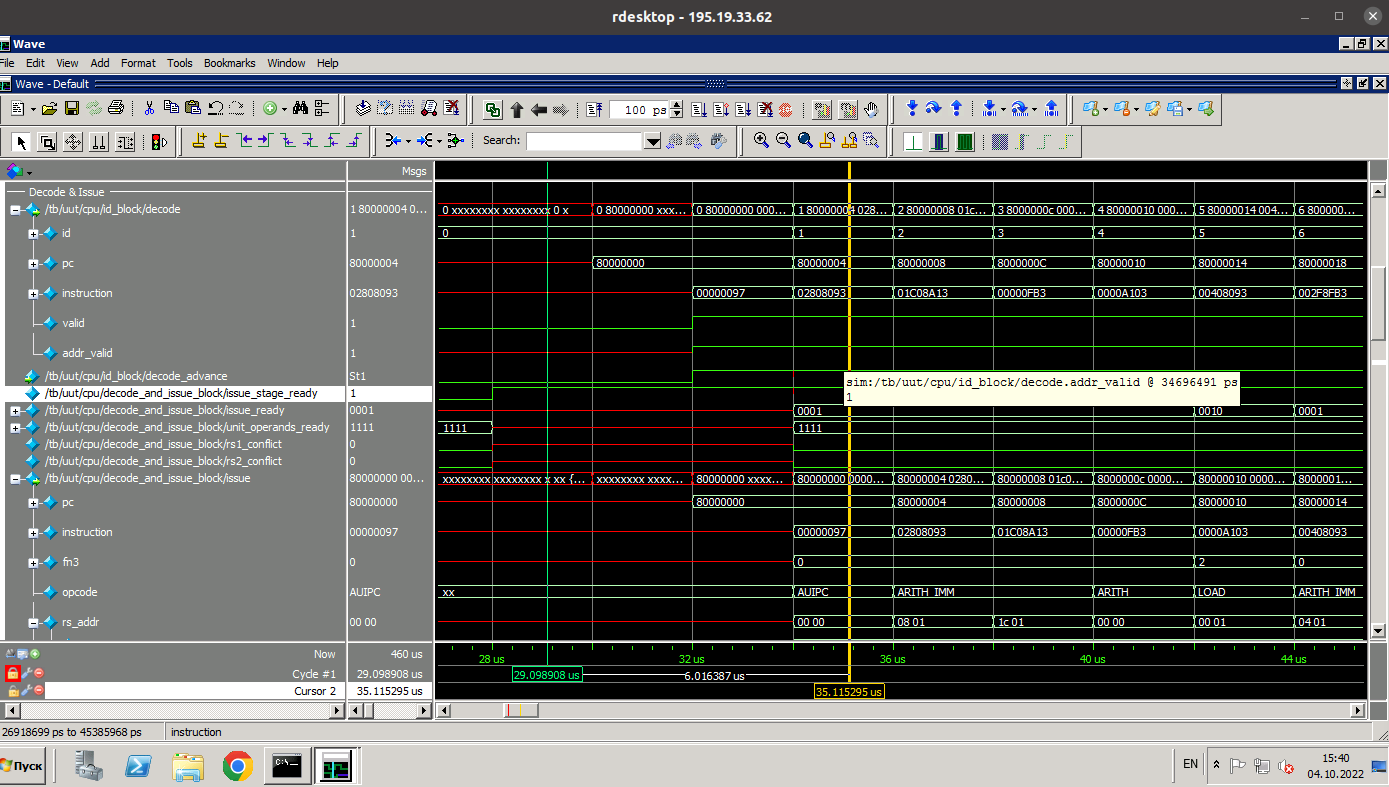
\includegraphics[width = \linewidth]{img/var4task5decode.png}
	\caption{Временная диаграмма выполнения стадий декодирования, планирования на выполнение и выполнения команды с адресом 80000010}
	\label{var4task5decode}
\end{figure}
\newpage
\section{Трасса выполнения программы}
В результате анализа диаграммы была заполнена трасса выполнения программы. Трасса выполнения показана на рисунке \ref{not_opt} \newpage

\begin{figure}[h]
	\centering
	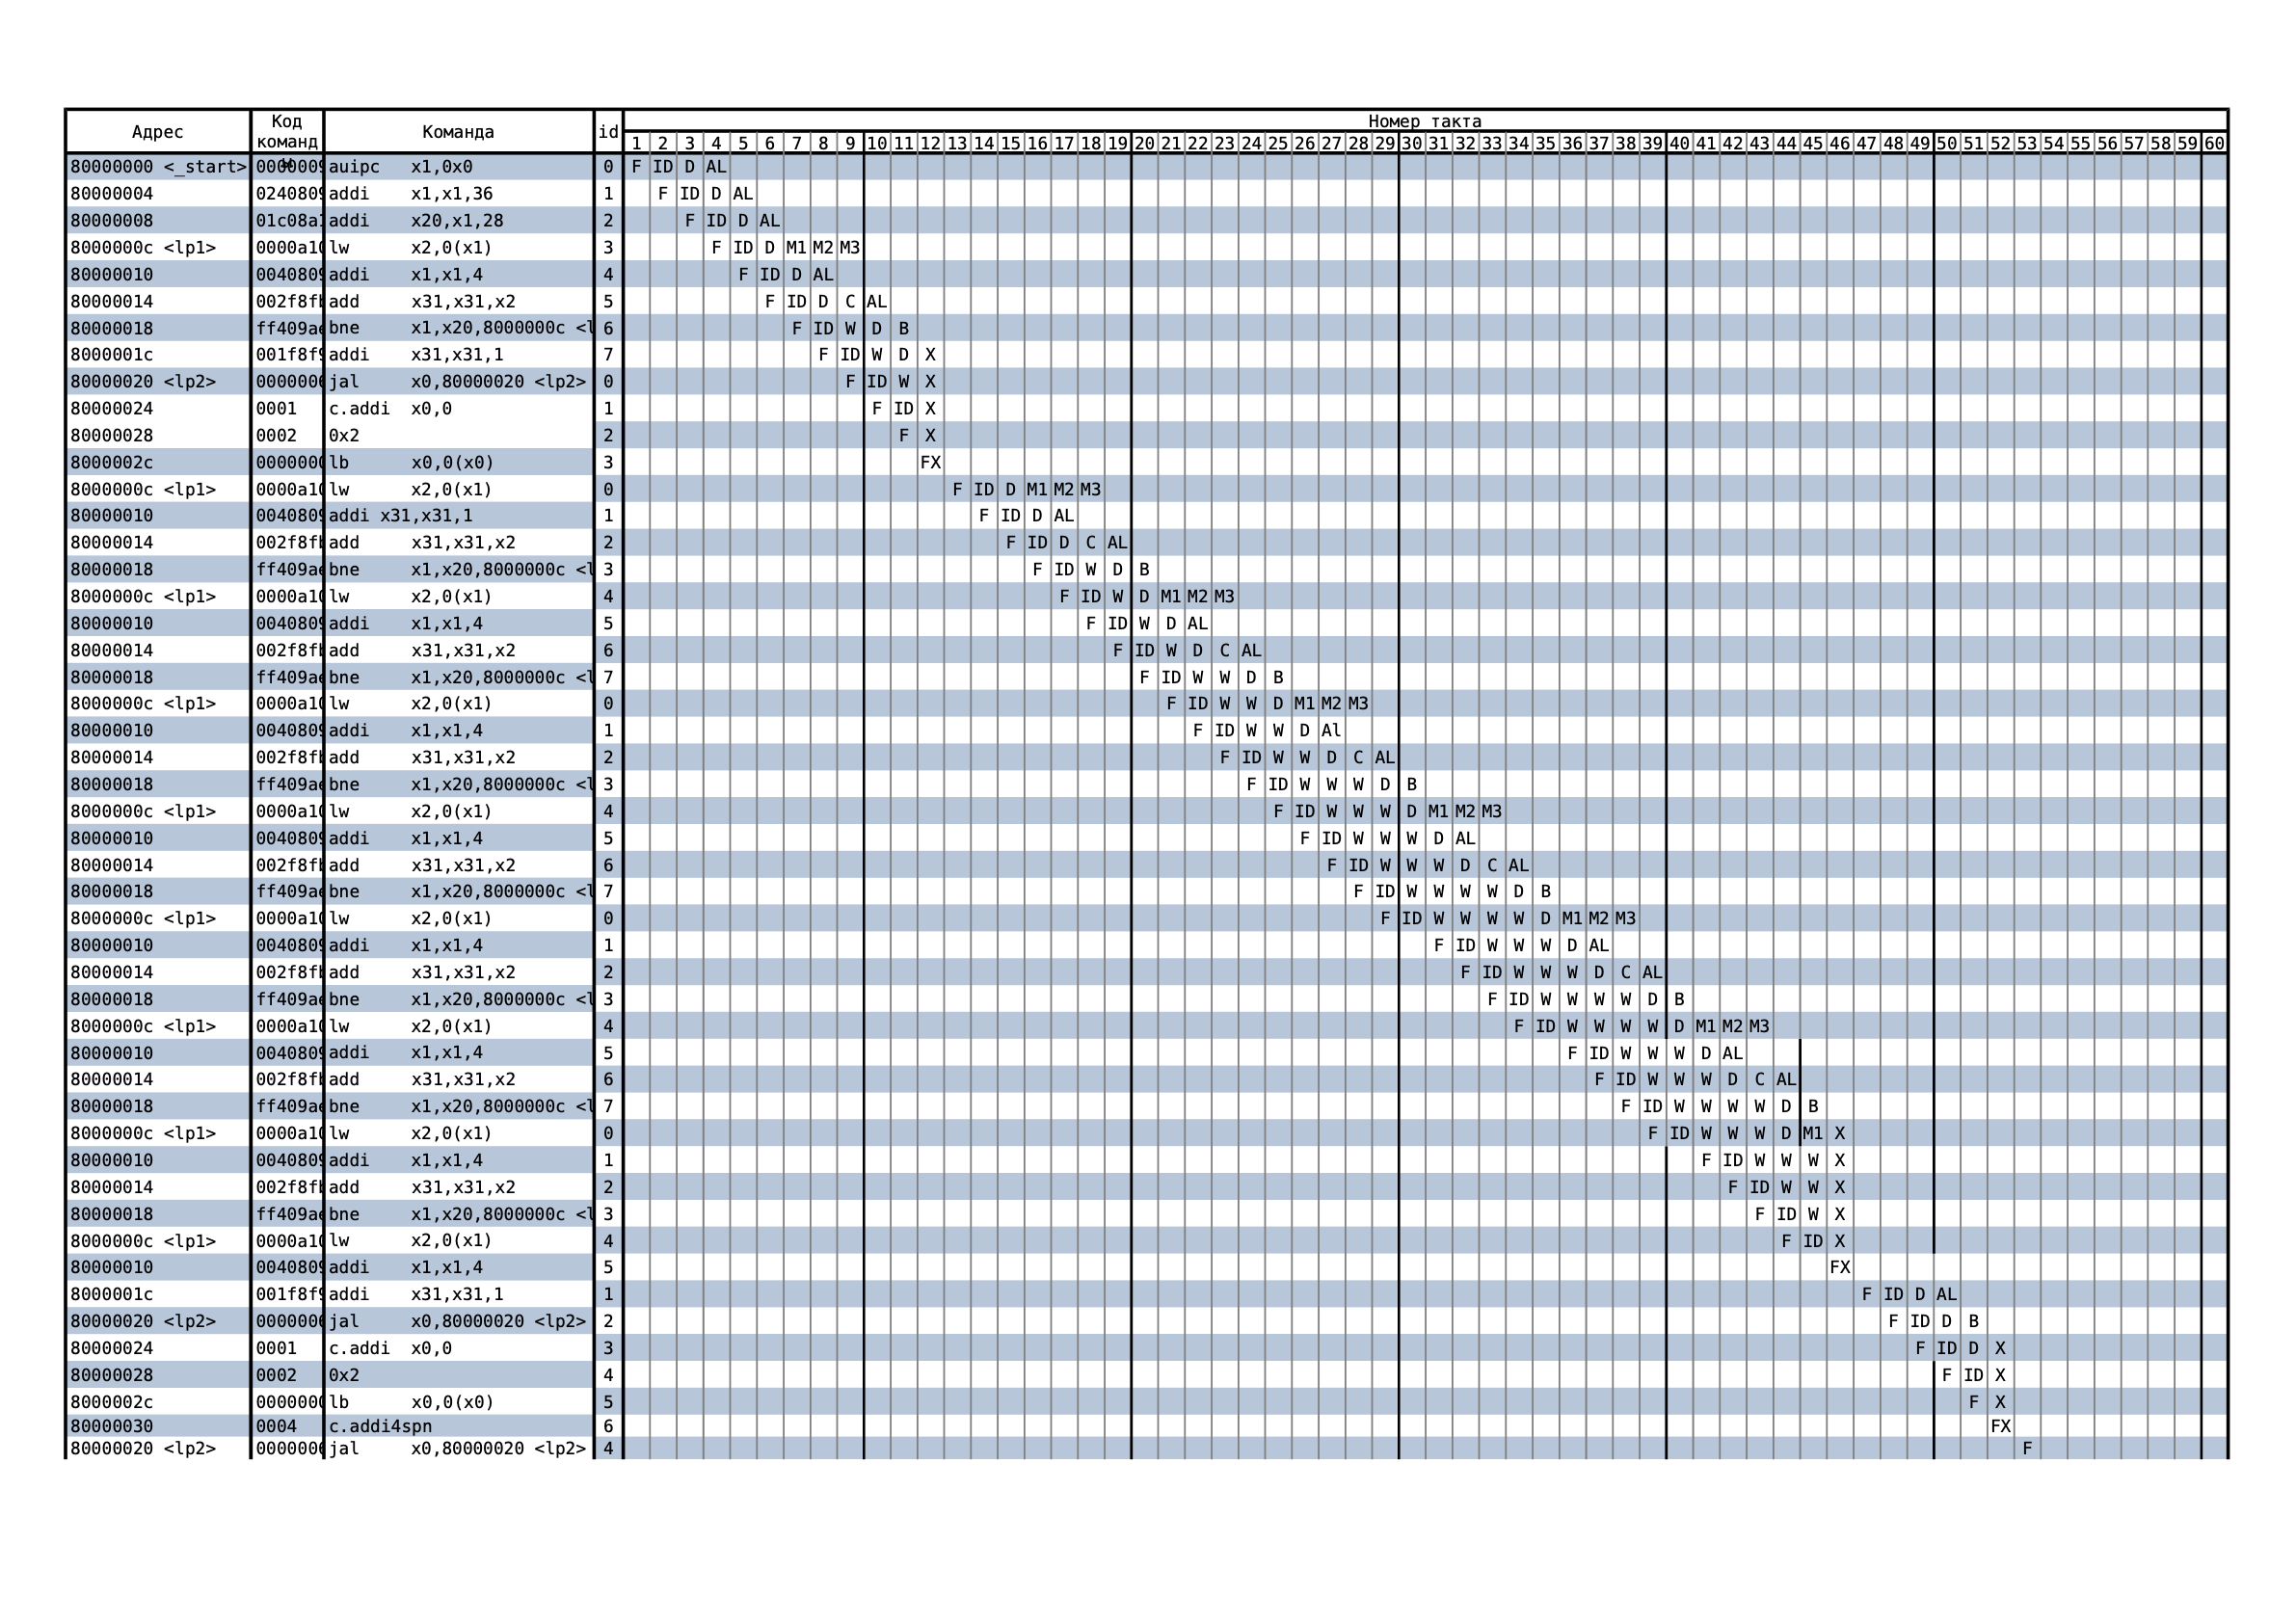
\includegraphics[width = \linewidth]{img/not_opt.png}
	\caption{Трасса выполнения программы}
	\label{not_opt}
\end{figure}

\section{Оптимизация программы}
Из анализа программы видно, что отсутствует возможность сократить время выполнения путем перестановки команд для ликвидации конфликтов и ожиданий декодера.

\section*{Вывод}
\addcontentsline{toc}{section}{Вывод}
Выполняемая программа имеет оптимальный порядок команд и не нуждается в оптимизации. 

